\subsubsection{Dirbtinis neuronas, perceptronas}

Šiame darbe nagrinėjami dirbtiniai neuroniniai tinklai yra sudaryti iš Rosenblato darbe \cite{rosenPerc} aprašytų dirbtinių neuronų, perceptronų. Perceptronas -  tai iteratyviai apmokomas tiesinis klasifikatorius, kuris susideda iš $\boldsymbol{x} = \{x_{0}1, x_{1}, x_{2}, ..., x_{p}\}$ mokymo aibės, kurios dydis yra n, vektorių, vadinamais įėjimais, $\{w_{0}, w_{1}, w_{2}, ..., w_{p}\} \in \R$ perdavimo koeficientų, vadinamų svoriais, aktyvacijos (perdavimo) funkcijos $f(a)$ ir $\{y_{0}, y_{1}, y_{2}, ..., y_{n}\}$ reikšmių, vadinamų išėjimais. Įėjimas $x_{0}$ yra vadinamas nuliniu įėjimu ir jo reikšmė yra pastovi $x_{0} = 1$, o $w_{0}$ - nuliniu svoriu arba slenksčiu (angl. bias). Perceptronas yra atvaizduotas paveikslėlyje \ref{img:perceptron}

\begin{figure}[H]
	\centering
	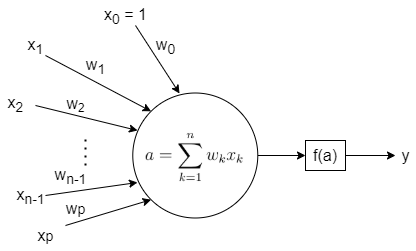
\includegraphics[scale=0.5]{img/perceptron.png}
	\caption{Perceptronas}
	\label{img:perceptron}
\end{figure}

Formulė \ref{eqn:activ_arg} yra aktyvacijos funkcijos argumentas.

\begin{equation}
	\label{eqn:activ_arg}
	a = \sum_{k = 1}^{p} w_{k}x_k
\end{equation}

Dažniausiai perceptronui yra naudojamos šios aktyvacijos funkcijos: slenkstinė (angl. unit step) \ref{eqn:unitStep}, sigmoidinė (angl. sigmoid) \ref{eqn:sigmoid}, gabalais tiesinė (angl. piecewise linear) \ref{eqn:pieceLinear}, Gauso (angl. Gaussian) \ref{eqn:gaussian} ir tiesinė (angl. linear) \ref{eqn:linear}

\begin{equation}
	\label{eqn:unitStep}
	f(a) =
	\begin{cases}
		0, & \mbox{jei } \beta > a \\
		1, & \mbox{jei } \beta \leq a
	\end{cases}
\end{equation}

\begin{equation}
	\label{eqn:sigmoid}
	f(a) = \dfrac{1}{1 + \exp^{-\beta }}
\end{equation}

\begin{equation}
	\label{eqn:pieceLinear}
	f(a) =
	\begin{cases}
		0, & \mbox{jei } a_{min} \geq  \\
		ma + b, & \mbox{jei } a_{min} < a < a_{max} \\
		1, & \mbox{jei } a_{max} \leq a
	\end{cases}
\end{equation}

\begin{equation}
	\label{eqn:gaussian}
	f(a) = \dfrac{1}{\sqrt{2\pi\sigma}} \exp^{\dfrac{-(a - \mu)^2}{2\sigma^2}}
\end{equation}

\begin{equation}
	\label{eqn:linear}
	f(a) = ma + b
\end{equation}

Perceptronas yra skirtas spręsti klasifikavimo uždavinius. Tam kad perceptronas spręstų konkretų klasifikavimo uždavinį, jis turi būti apmokytas. Perceptrono apmokymas yra iteratyvus procesas, kuriame randami svoriai $W = \{w_{0}, w_{1}, w_{2}, ..., w_{n}\}$, su kuriais funkcijos \ref{eqn:mse} rezultatas įgyja apytiksliai mažiausią reikšmę. Funkcijoje \ref{eqn:mse} $y_i$ yra perceptrono i-tasis išėjimas ir $t_i$ - i-tojo įėjimo norima klasė.

\begin{equation}
	\label{eqn:mse}
	e(w) = \dfrac{1}{n}\sum_{i=1}^{n}(y_i - t_i)^2
\end{equation}

Apmokymo pradžioje pradiniai svoriai yra parenkami atsitiktinai. Toliau gradientinio nusileidimo algoritmu judant antigradiento kryptimi, svorių reikšmės perskaičiuojamos naudojantis funkcija \ref{eqn:w_recalc}, kur $\Delta w_k(t)$ yra funkcija \ref{eqn:w_change}, $t$ - iteracijos numeris, $\eta \in [0, +\infty]$ - parinktas mokymo greitis (angl. learning rate), ir vieną įėjimo vektorių iš duomenų aibės. Svoriai yra perskaičiuojami norima skaičių kartų.

\begin{equation}
	\label{eqn:w_recalc}
	w_k(t + 1) = w_k(t) + \Delta w_k(t)
\end{equation}

\begin{equation}
	\label{eqn:w_change}
	\Delta w_k(t) = - \eta \dfrac{\partial e(w)}{\partial w_k}
\end{equation}
% išsivedamas bendras atvejis ------------------------------------------------------------------------------------------------------------------------
Pakeitus, kai kurių kintamųjų žymėjimą, iš lygties \ref{eqn:activ_arg} gaunama lygtis \ref{eqn:activ_arg_per_i}, kur $a_i$ yra i-tojo įėjimo vektoriaus aktyvacijos funkcijos argumentas, $x_{ik}$ yra i-tojo įėjimo vektoriaus k-atoji komponentė.

\begin{equation}
	\label{eqn:activ_arg_per_i}
	a_i = \sum_{k = 1}^{p} w_{k}x_{ik}
\end{equation}

Tad i-tasis perceptrono išėjimas $y_i$ yra $y_i = f(a_i)$. Tada funkcijos \ref{eqn:mse} išvestinė yra lygtis \ref{eqn:expanded}.

\begin{equation}
	\label{eqn:expanded}
	\dfrac{\partial e(w)}{\partial w_k} = (\dfrac{1}{n}\sum_{i=1}^{n} (y_i - t_i)^2)'
		= \dfrac{2}{n}\sum_{i=1}^{n}
			((y_i - t_i)(f'(a_i))(\sum_{k = 1}^{p} x_{ik}))
\end{equation}

Tada bendru atveju perceptrono mokymo taisyklė \ref{eqn:w_recalc} yra funkcija \ref{eqn:general}.

\begin{equation}
	\label{eqn:general}
	w_k(t + 1) = w_k(t) - \eta \dfrac{2}{n}\sum_{i=1}^{n} ((y_i - t_i)(f'(a_i))(\sum_{k = 1}^{p} x_{ik}))
\end{equation}

% išsivedamas bendras atvejis ------------------------------------------------------------------------------------------------------------------------
Naudojantis apmokytu perceptronu galima nustatyti duoto duomenų vektoriaus $\boldsymbol{x}'$ klasę. Klasė nustatoma randant reikšmę $a$ iš lygties \ref{eqn:activ_arg}, kur $\{w_{0}, w_{1}, w_{2}, ..., w_{p}\}$ yra apmokyto perceptrono svoriai ir $\{x_{0}, x_{1}, x_{2}, ..., x_{p}\} = \boldsymbol{x}'$. $\boldsymbol{x}'$ vektoriaus klasė atitiks intervalo $b_c$, į kurį patenka reikšmė $a$, klasė $c$. Klasių intervalai $b_c \in \R$ yra paskaičiuojami, padalinant $\R$ su skiriamuoju paviršiumi (angl. decision boundary), o skiriamasis paviršius yra nustatomas pagal aktyvacijos funkciją.
